\subsection{Tamaño del conjunto de entrenamiento}\label{fer}
En la sección anterior arribamos a la conclusión de cuáles son los intervalos óptimos para los parámetros de cada una de las técnicas. Más aún, escogimos los exponentes de estos rangos; aquellos valores de \emph{k} para \emph{kNN} y de $\alpha$ para \emph{PCA} que maximizan alguna de las métricas; en nuestro caso particular, fijamos la atención en el \emph{accuracy}. 
\par
Ahora bien, esta elección se basa en los resultados y el análisis de un experimento llevado a cabo sobre un conjunto de datos de un tamaño determinado. Entonces, surge la necesidad de corroborar la calidad óptima de estos valores al ser utilizados con conjuntos de entrenamiento de otras dimensiones. Es de interés observar si se produce un corrimiento de los intervalos previamente encontrados; o bien, si los exponentes de éstos continúan maximizando el \emph{accuracy}. 
\par
Con el fin de encontrar una respuesta a estas intrigas, planteamos una generalización del experimento hecho en la sección previa; variando -además- la cantidad de elementos que constituyen al conjunto de entrenamiento. Adicionalmente, ampliamos los rangos de los argumentos de las técnicas sobre los cuales experimentamos, para poder observar posibles movimientos de los intervalos óptimos. Nuevamente, para que la evaluación de las predicciones resulte más robusta se realizó validación cruzada con 10 \emph{folds}.
\par
A partir de los resultados obtenidos pudimos identificar tres dimensiones para analizar. En primer lugar, estudiamos el comportamiento de los valores óptimos para los parámetros de cada técnica a medida que varía el tamaño del conjunto de entrenamiento; lo que originalmente motivó a hacer el experimento. Luego, la relación entre la calidad de las predicciones y las dimensiones del conjunto; y finalmente, el costo temporal en relación a éste. En las siguientes secciones discutimos cada uno de estos aspectos con mayor detalle.

\subsubsection{Argumentos óptimos}
Retomamos la motivación original de esta sección: observar si los valores óptimos previamente encontrados dependen del tamaño del conjunto con el cual se entrena al predictor. Hay un especial interés en responder las siguientes preguntas: aquellos argumentos que maximizan el \emph{accuracy} para el conjunto utilizado en la sección anterior, ¿continuarán maximizando las métricas? En caso de no ser así, ¿seguirán siendo efectivos? A pesar de que se pueda perder calidad en los resultados, ¿podremos usarlos independientemente de la cantidad de datos de entrenamiento?
\par
\begin{figure}[h]
    \centering
    \subfloat{{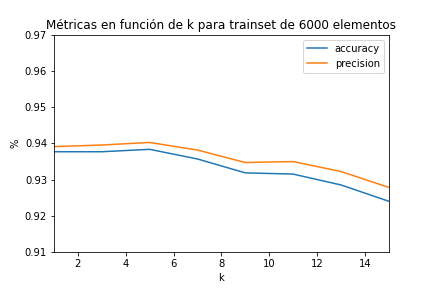
\includegraphics[width=.4\linewidth]{images/tamanio/metricas_knn_6000.png} }}%
    \subfloat{{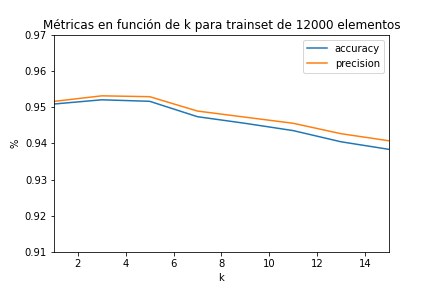
\includegraphics[width=.4\linewidth]{images/tamanio/metricas_knn_12000.png} }}%
    
    \subfloat{{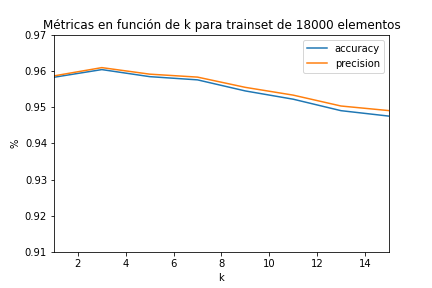
\includegraphics[width=.4\linewidth]{images/tamanio/metricas_knn_18000.png} }}%
    \subfloat{{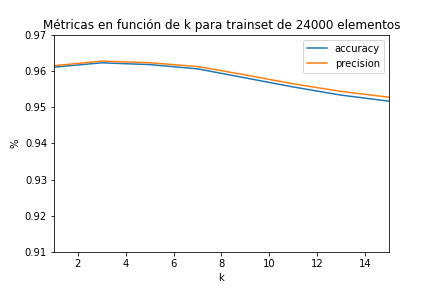
\includegraphics[width=.4\linewidth]{images/tamanio/metricas_knn_24000.png} }}%
    
    \subfloat{{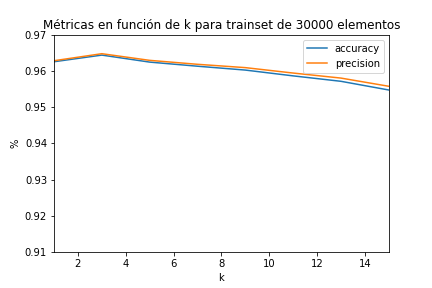
\includegraphics[width=.4\linewidth]{images/tamanio/metricas_knn_30000.png} }}%
    \subfloat{{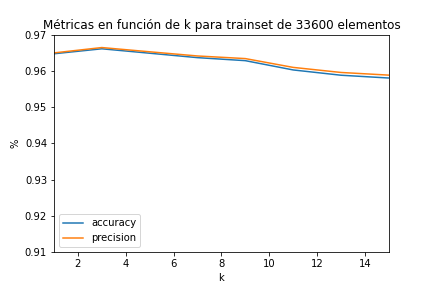
\includegraphics[width=.4\linewidth]{images/tamanio/metricas_knn_33600.png} }}%
    
    \caption{Métricas knn en función de k}
    \label{fig:metricas_knn}
\end{figure}
\par
Las figuras en \ref{fig:metricas_knn} muestran los resultados obtenidos para el caso donde se utiliza \emph{kNN} de manera individual. Cada una expone las métricas de \emph{accuracy} y \emph{precision} en función del parámetro \emph{k} para un conjunto de entrenamiento de tamaño determinado. A simple vista, notamos que ambas métricas presentan un comportamiento bastante similar; entonces, nos reducimos a discutir los resultados obtenidos desde el punto de vista del \emph{accuracy}. Luego, con la información expuesta podemos hacer dos observaciones principales. Por un lado, notamos que en todos los casos el intervalo óptimo para los valores de \emph{k} se posiciona entre los números $[1, 7]$. Esto nos da un indicio de que existe una suerte de relación independiente entre el tamaño del conjunto de entrenamiento y el rango óptimo de argumentos para \emph{kNN}. Por otro lado, vemos que conforme crece el tamaño del conjunto, el valor de \emph{k} que maximiza las métricas se va corriendo del 5 al 3. Particularmente, cuando el tamaño es 6000, el valor óptimo es 5; cuando éste es 12000, notamos una suerte de empate entre 3 y 5; y a partir de 18000, las métricas muestran mejores resultados con \emph{k} igual a 3. Con esto podemos dar una mínima garantía de que utilizar \emph{kNN} con un $k=3$ continúa siendo una elección adecuada independientemente de la cantidad de datos con la que se lo entrene. En la mayoría de los casos las mejores predicciones se encuentran asociadas a este argumento. Notemos, que el el caso particular donde el argumento óptimo resultó ser $k=5$, la diferencia entre las métricas para 3 y 5 no es del todo significativa. No obstante, esto último va a terminar dependiendo del área de aplicación. Finalemnte, esto deja la siguiente intriga: ¿qué ocurre cuando \emph{k} vale 4? Recordemos que experimentamos únicamente con los valores impares del intervalo $[1,15]$. Quizás, deberíamos reiterar el experimento con el intervalo $[1,7]$ y aumentar la granularidad.
\par
\begin{figure}[h]
    \centering
    \subfloat{{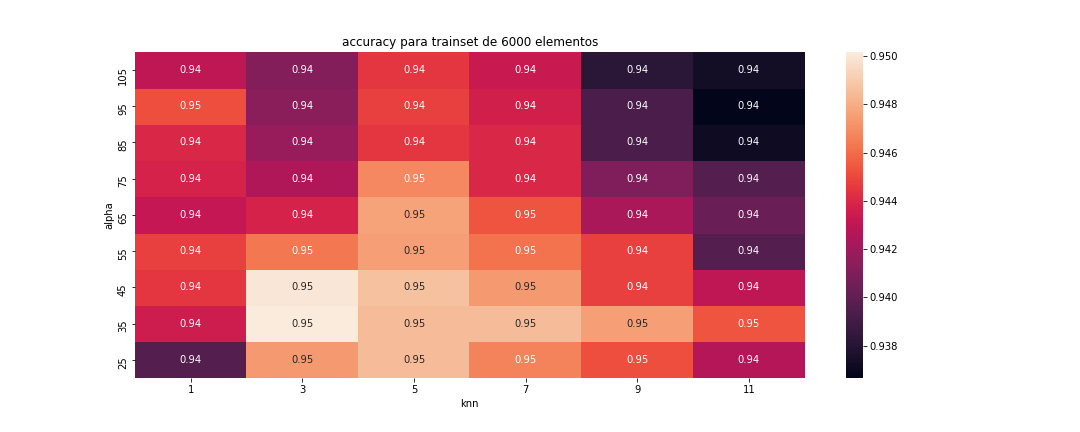
\includegraphics[width=.5\linewidth]{images/tamanio/metricas_knn_pca_6000.png} }}%
    \subfloat{{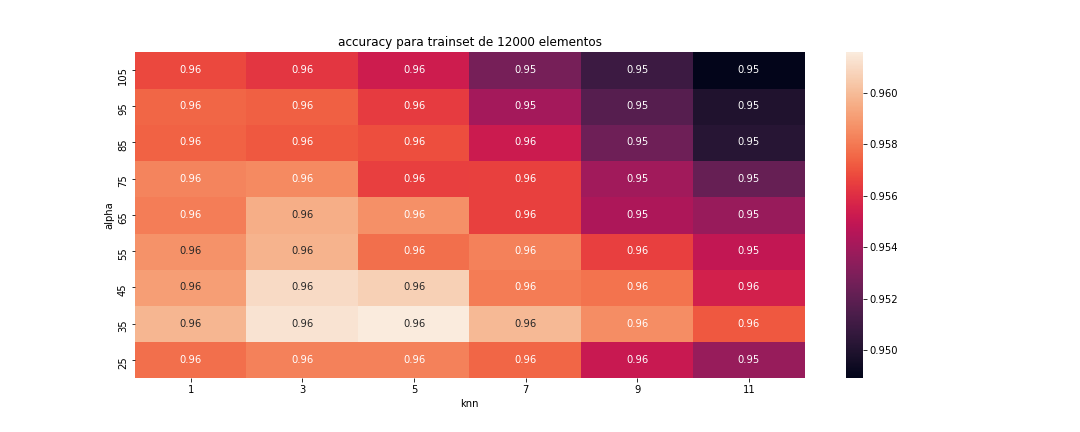
\includegraphics[width=.5\linewidth]{images/tamanio/metricas_knn_pca_12000.png} }}%
    
    \subfloat{{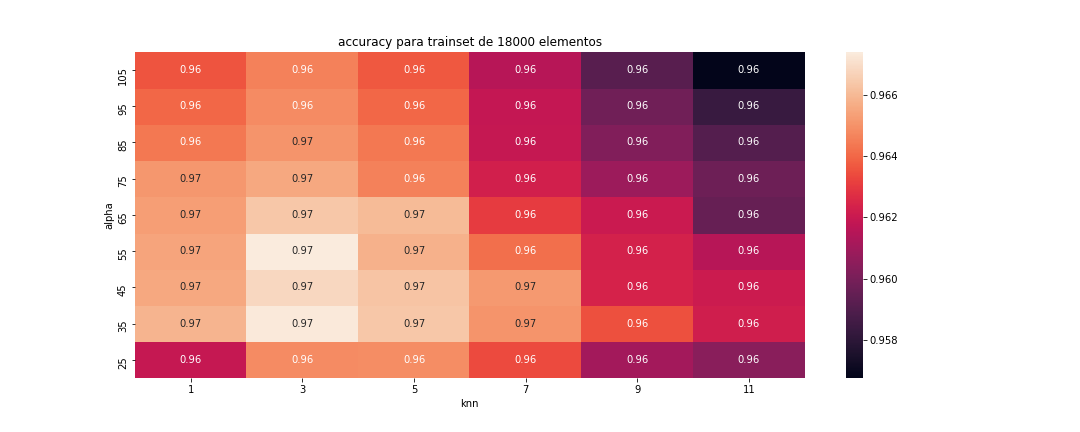
\includegraphics[width=.5\linewidth]{images/tamanio/metricas_knn_pca_18000.png} }}%
    \subfloat{{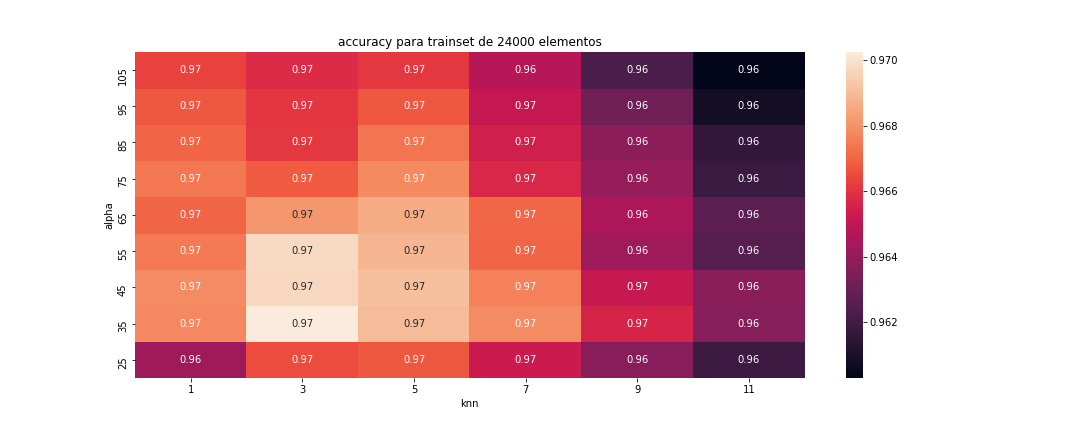
\includegraphics[width=.5\linewidth]{images/tamanio/metricas_knn_pca_24000.png} }}%
    
    \subfloat{{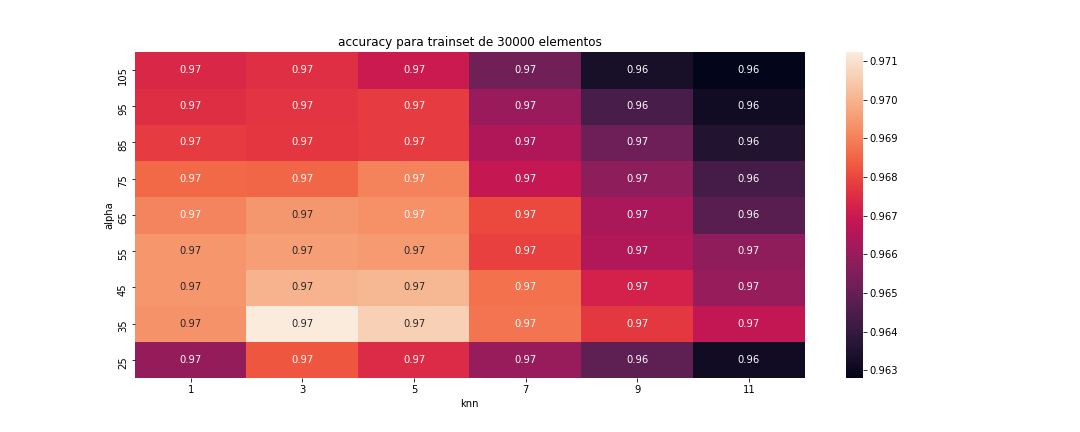
\includegraphics[width=.5\linewidth]{images/tamanio/metricas_knn_pca_30000.png} }}%
    \subfloat{{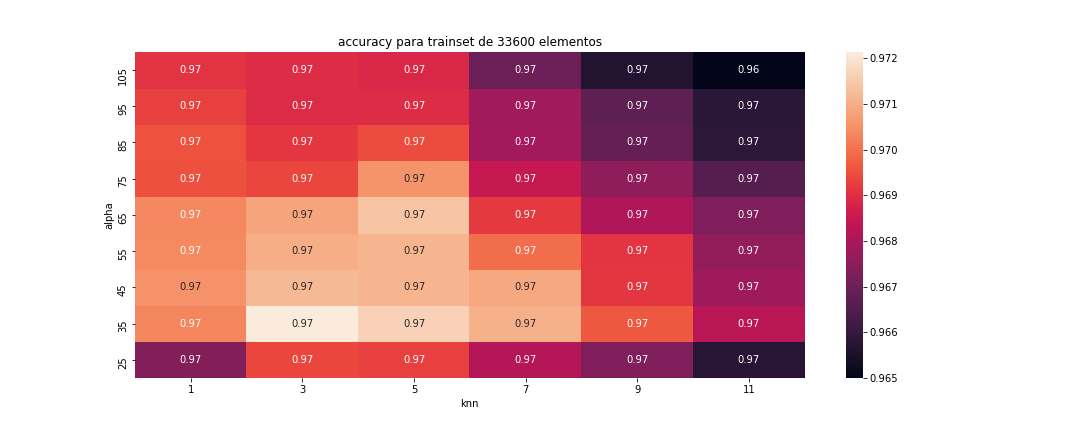
\includegraphics[width=.5\linewidth]{images/tamanio/metricas_knn_pca_33600.png} }}%
    
    \caption{Métricas knn-pca en función de k y alpha}
    \label{fig:metricas_knn_pca}
\end{figure}
\par
Luego, en las figuras en \ref{fig:metricas_knn_pca} se presentan la evaluación de los resultados obtenidos al combinar \emph{PCA} con \emph{kNN}. Como mencionamos en le párrafo anterior, escogimos exponer únicamente el caso del \emph{accuracy} debido a la semejanza en el comportamiento con las demás métricas. Estos mapas de calor muestran el \emph{accuracy} calculado para cada combinación de los parámetros \emph{k} y $\alpha$. Escogimos utilizar mapas de calor para poder observar qué forma tomaba el intervalo de parejas óptimas alrededor del mejor exponente. En primer lugar, observamos que los intervalos óptimos no se corrieron al variar el tamaño del conjunto de entrenamiento. Además, podemos ver que la pareja óptima converge a (\emph{k}=3, $\alpha=$35) conforme crece el tamaño. Concretamente, a partir de 18000, ya converge. Por lo tanto, podemos suponer que nuestra elección de pareja óptima también aplica para otros tamaños de \emph{trainset}; no necesariamente maximizará el \emph{accuracy} en todos los casos, pero si se mantendrá bastante cerca de la pareja en \emph{primer lugar}. Notemos que en la sección anterior se concluyó que esta era (4, 40). Sin embargo, cabe aclarar que en este experimento se decidió probar con los valores impares de los rangos, a diferencia del experimento previo, donde se prestó atención a los pares. De todas formas, vemos que (3,35) y (4,40) son parejas \emph{hermanas} si tenemos en cuenta el tema de paridad en conjunción con los incrementos de 10 unidades en el caso del $\alpha$. Aún así, surge la necesidad de experimentar con mayor granularidad en torno a estas parejas.
\par
Entonces, con el análisis en esta primera sección podemos aportar una mínima garantía al supuesto de relación independiente entre los argumentos óptimos de las técnicas y las dimensiones del conjunto de entrenamiento.

\subsubsection{Calidad de las predicciones}
En esta sección hacemos un pequeño análisis de la calidad de los resultados generados por cada técnica a medida que varía el tamaño del conjunto de entrenamiento. En primer lugar, estudiamos el comportamiento de algunas métricas para cada técnica por separado. Luego, las comparamos entre sí. Se intentan responder preguntas como: ¿Cómo se relacionan la técnicas con el tamaño del conjunto de entrenamiento? ¿Podemos jerarquizar las técnicas? ¿Habrá tamaños para los cuales una es más adecuada que la otra?
\par
Teniendo en cuenta el análisis de la sección [sección argumentos óptimos], decidimos estudiar únicamente los resultados generados por los argumentos que maximizan las métricas. Particularmente $k=3$ y $\alpha=35$.
\par
\begin{figure}[h]
 \centering
 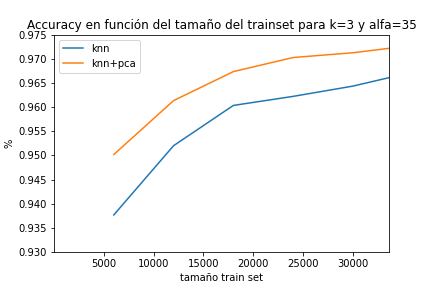
\includegraphics[width=.7\linewidth]{images/tamanio/metricas_comparacion.png}
 \caption{Comparación de métricas}
 \label{fig:metricas_comp}
\end{figure}
\par 
La figura \ref{fig:metricas_comp} expone la evaluación de los resultados obtenidos por cada técnica en relación a la cantidad de datos con la cual se entrenó. Podemos observar que para las técnicas la relación entre la calidad de las predicciones y el tamaño del conjunto de entrenamiento es proporcional. Además notamos que el crecimiento en función del tamaño es similar en ambos casos. Creemos que la razón de esto radica en que conforme crece la cantidad de datos de entrenamiento se tienen más instancias de cada clase; particularmente, de la clase relevante a una predicción determinada. Luego, cuando se busquen los $k$ vecinos más cercanos a la entrada, habrá una mayor probabilidad de que las instancias parecidas a la entrada que pertenezcan a la clase relevante. Ahora bien, esto se cumple bajo el supuesto de que conforme crece el conjunto de entrenamiento se mantiene un cierto balance entre las distintas clases y que la mayoría de las instancias se encuentra bien definida. Por otro lado, vemos que la relación entre calidad y tamaño del conjunto no es necesariamente lineal: a partir del 18000 el crecimiento resulta ser menos drástico.
\par
Si bien presentan una curva de crecimiento similar, notamos una clara diferencia entre los valores concretos de cada técnica. Para todos los conjuntos de entrenamiento hay una diferencia de aproximadamente 0,1 entre los valores de \emph{accuracy} de cada una; en todos los casos, se favorece a la combinación de \emph{PCA} y \emph{kNN}. Entonces, pareciera ser que la utilización de \emph{PCA} para reducir redundancias entre los datos del conjunto de entrenamiento y maximizar la varianza de éstos tiene como efecto que las predicciones realizadas con \emph{kNN} resulten más acertadas en el caso general. Más aún, destacamos la posibilidad de que esta mejora en la calidad de los resultados se mantenga constante independiente de la cantidad de datos con la que se entrena.
\par
Cerrando esta sección, concluimos que la calidad de las predicciones aumenta a la par con el tamaño del conjunto de entrenamiento; y que el crecimiento observable es similar en ambos casos. Luego, notamos una clara mejora al combinar \emph{PCA} con \emph{kNN}.

\subsubsection{Costo temporal}
Habiendo establecido que aplicar \emph{PCA} sobre los datos antes de predecir con \emph{kNN} genera resultados de mayor calidad, surge la necesidad de estudiar el costo temporal asociado a la presencia o a la ausencia de \emph{PCA}. A simple no podemos observar una jerarquía muy obvia. En ambos casos hay motivos para creer que una será consumira menos tiempo que la otra. Por un lado, tenemos que el uso de \emph{PCA} implica la neceisadad de calcular una serie de autovector y autovalores, lo cual -aplicando el metodo de la potencia- podría implicar un costo adicional no trivial. Por el otro lado, tenemos que los datos resultantes de haberles aplicado la transformación asociada son de menor dimensión.Esto podría implicar una reducción en el timpo de ejecución de \emph{kNN}; notamos la relación directa entre las dimensiones del conjunto de entrenamiento y el costo temporal de buscar los vecinos más cercanos.
\par
Con los tiempos obtenidos de cronometrar las distintas corridas del experimento construimos las figuras \ref{fig:tiempo_pred}. La figura de la izquierda muestra únicamente los tiempos de ejecución asociados a la función de predicción de las dos variantes; mientras que en la figura de la derecha se incluye el costo asociado a aplicar la técnica \emph{PCA}. Curiosamente, notamos que en ambos casos la diferencia entre los costos temporales se va haciendo cada vez más significativa conforme aumenta el tamaño del \emph{set} de entrenamiento. La reducción en la dimensión pareciera ser un factor de gran importancia para el tiempo de ejecución. Además, vemos que los cálculos asociados a \emph{PCA} no demuestran ser lo suficientemente altos como para generar una suerte de \emph{trade-off} entre la calidad de los resultados y el costo temporal. El único caso donde supera a la versión individual de \emph{kNN} es cuando el tamaño del \emph{trainset} es muy pequeño. Sin embarge, conforme aumenta la cantidad de datos de entrenamiento, el costo asociado a las predicciones luego de haber utilizado \emph{PCA} no crece de manera drástica; en contraposición a la otra versión.
\par
En suma, podemos concluir que la combinación de \emph{PCA} con \emph{kNN} representa una mejora no trivial tanto en la calidad de las predicciones como en el costo temporal de la técnica. 

\begin{figure}[h]
    \centering
    \subfloat{{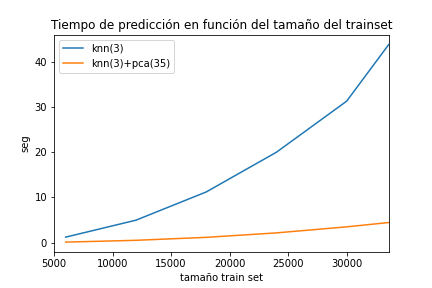
\includegraphics[width=.5\linewidth]{images/tamanio/tiempos_pred.png} }}%
    \subfloat{{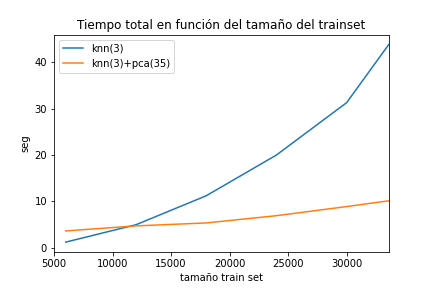
\includegraphics[width=.5\linewidth]{images/tamanio/tiempos_total.png} }}%
    
    \caption{Tiempo de predicción en función del tamaño}
    \label{fig:tiempo_pred}
\end{figure}
